\chapter{序論}
\thispagestyle{empty}
\label{chap1}
\graphicspath{{chap1/figure/}}
\minitoc

%%%%%%%%%%%%%%%%%%%%%%%%%%%%%%%%%%%%%%%%%%%%%%%%%%%%%%%%%%%%%%%%%%%%%%%%%%%%

% ================================================== %
% section
% ================================================== %
\newpage
\section{X線天文分野におけるミラー結像系}
\label{chap1_imaging_mirror_in_astronomy}

太陽の活動を理解することは、天文分野において重要な意味を持ち、未だに残る多くの謎に対して現在も多くの努力がなされている。
中でも、太陽の中心核から光球に向かって6000℃まで温度が下がっていくのに対し、そこからはるか上空にあるコロナが100万℃の高温状態であるというパラドクスは「コロナ加熱問題」として知られる。
他の銀河系における高温プラズマ発生の原理解明にも繋がるため、重要な問題として位置づけられている。\cite{ShimizuToshifumi2018}
これらの現象は、高温なプラズマから放射されるX線領域の電磁波を検出することで観測できる。
静穏な領域は数百eVから1keV以下の軟X線領域に、活発な領域は数keVから数十keVの硬X線領域にそれぞれ対応する。
このようなX線領域の天体観測においては、効率と受光面積の観点からミラーによる結像系が用いられる。
X線は大気によって吸収されやすいため、太陽コロナのX線領域での観察は大気圏外に打ち上げられた宇宙船上で行われるのが望ましい。
ロケットにミラー結像系を搭載し対象の現象を撮影するには、飛行中の振動に耐えなければならない。
また、コロナ加熱問題を含む種々の現象を解明するためには活動領域の経時的な変化を追う必要があり、観測中の一貫した安定性が求められる。

\clearpage
% -------------------------------------------------- %
% section
% -------------------------------------------------- %
\newpage

\section{Wolterミラー}
\label{chap1_wolter_mirror}

外乱に強く安定した結像の実現という要求に対して有用なのが、Wolterミラーである。\cite{1952AnP...445...94W}

十分遠方にある天体を観測する際、それが発するまたは反射する光はほぼ平行光とみなせる。
放物線の持つ平行光線を反射して焦点に集めるという効果を利用して、放物線を軸回りに回転した曲面により平行光を1点に集める光学素子が回転放物面ミラーである。
全周に渡って回転した回転放物面ミラーは、円形に広がる平行光に対してこれを1点に集光する。

しかし、回転放物面には設置角度の誤差に弱いという欠点が存在する。
これを解決するのが、2回の反射により結像を行うWolterミラーである。
図\ref{fig:wolter_robustness}に示すように、2回反射ミラーでは最終的に出射される光の進行角度が設置角度誤差の影響を受けない。

\begin{figure}[b]
\centering
\caption{2回反射による設置角度誤差のキャンセル}
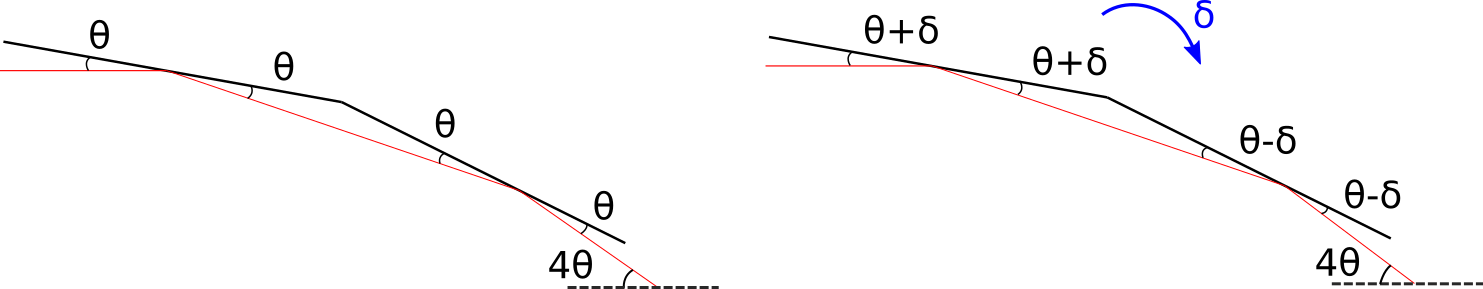
\includegraphics[width=10cm]{wolter_robustness.png}
\label{fig:wolter_robustness}
\end{figure}

Wolterミラーは近似的にAbbeの正弦条件を満たし、無限遠方でのより広い領域に対して鮮明な像を結ぶ。\cite{VanSpeybroeck1972}

Wolterミラーの形状は、2種類の2次曲線を組み合わせた図形の回転体として与えられる。
焦点を共有するように2つの2次曲線を配置することで、平行光を1点に集光する光学素子となる。
WolterミラーにはI型(図\ref{fig:wolter_type_1})・II型(図\ref{fig:wolter_type_2})・III型(図\ref{fig:wolter_type_3})の3種類が存在する。
それぞれの反射面は、I型が放物面内面・双曲面内面、II型が放物面内面・双曲面外面、III型が放物面外面・楕円面内面となっている。
I型は応用性が高く、最も利用されているWolterミラーとなる。
これは、2回とも内面で反射する構成であるため\ref{chap1_mirror_mandrel}節に述べるような凸形状から転写を行うマンドレル電鋳法が有効であることや、\ref{chap1_nested_wolter_mirror}節で述べるような複数枚のWolterミラーによるネスト構造を形成できる唯一の構成であることによる。
III型では2枚が重なるような配置が可能であり、焦点距離を短く設計し光学系全体を小型化できる。
しかし、I型に比べ加工・設置とも格段に難しくなるため、実用には至っていない。

\begin{figure}[b]
\centering
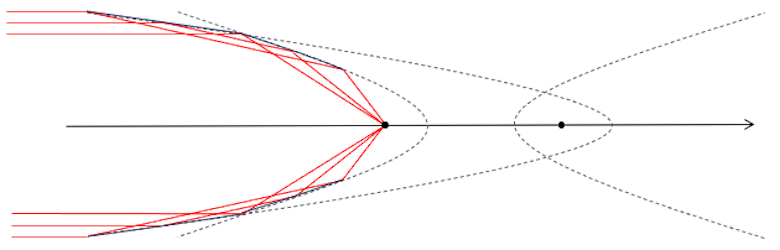
\includegraphics[width=10cm]{wolter_type_1.png}
\caption{Wolter I型}
\label{fig:wolter_type_1}
\end{figure}

\begin{figure}[b]
\centering
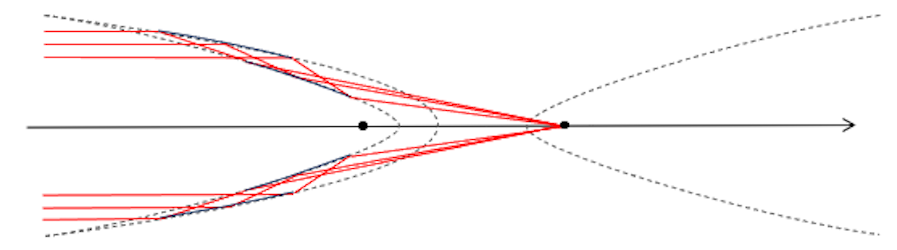
\includegraphics[width=10cm]{wolter_type_2.png}
\caption{Wolter II型}
\label{fig:wolter_type_2}
\end{figure}

\begin{figure}[b]
\centering
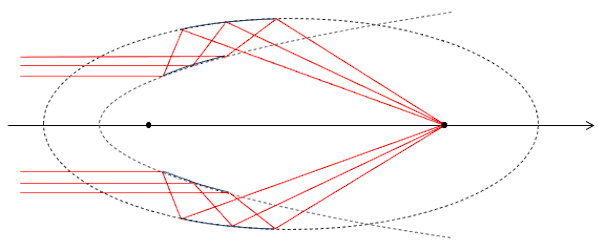
\includegraphics[width=10cm]{wolter_type_3.png}
\caption{Wolter III型}
\label{fig:wolter_type_3}
\end{figure}

\subsection{ネスト型Wolterミラー}
\label{chap1_nested_wolter_mirror}

Wolterミラーのような円筒形のミラー、特にX線を反射するため斜入射角が小さく設計されたミラーは、中空になっている内側部分を通過する光を集めることができず、集光強度を高める上で不都合である。
これを解決する方法として、図\ref{fig:nested_wolter_mirror}のように口径の異なるWolterミラーを内側に挿入するネスト構造がある。\cite{BuitragoCasas2017}

\begin{figure}[b]
\centering
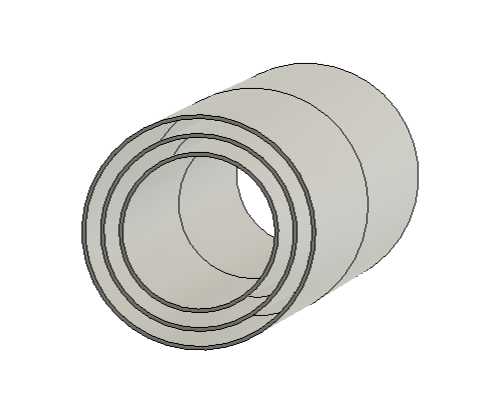
\includegraphics[width=8cm]{nested_wolter_mirror.png}
\caption{Nested Wolterミラーの例}
\label{fig:nested_wolter_mirror}
\end{figure}

ネスト構造を取ることで受光面積を大きくし、集光強度を上げることができる。
Wolterミラーでネスト構造を取ることができるのはI型のみであり、X線用結像光学系としてI型が最も有用である1つの理由となっている。
ネスト構造を構成することは受光面積の観点では有利だが、ミラー枚数を増やすほどその設置が困難になるという問題がある。
ミラー同士の角度・光軸のずれなど、調整しなければならない誤差要因が増えるためである。
そのため、ネスト構造の構成後に光学系を統合的に計測する方法が必要になる。
また、ミラー同士をネストさせたあとにプローブを挿入して計測することは困難であるため、その統合的な評価は間接測定によって行われなければならない。

\clearpage
% -------------------------------------------------- %
% section
% -------------------------------------------------- %
\newpage

\section{FOXSI4におけるWolterミラー}
\label{chap1_background}

\subsection{FOXSI}
\label{chap1_foxsi}

2018年に打ち上げられたFOXSI3では太陽コロナのX線写真を撮影することに成功した。\cite{weko_20796_1}
図\ref{fig:foxsi-fullsun-image}はその撮影像の1枚である。
1 秒間に 250 枚のデータを約 6 分間に渡って取得し、活動領域のX線について光子数の時間変化やスペクトルを算出した。
FOXSI3に続いて2023年頃に打ち上げが予定されているFOXSI4では、コロナ加熱問題の解決に関わるフレア現象の観測をターゲットとする。
太陽の状態を監視し、フレアの発生が検知された時点でロケットを打ち上げることで、フレアの中期から後期を観測することを目指している。
既にフレアの観測を行っているRHESSI\cite{Liu_2004}においては、撮影像の感度やダイナミックレンジが不十分であった。
これに対して、FOXSI4ではWolterミラーを用いた新たな結像系による鮮明な撮影像の取得が期待される。\cite{2019AGUFMSH31C3315V}
JAXAの進めるミッションLynxは、Wolterミラーの解像分解能の目標値をHPD 0.5 秒角と設定している\cite{Gaskin2019}。
FOXSI4に搭載予定のWolterミラーについても、同程度の目標を達成することが期待されている。

\begin{figure}[h]
\centering
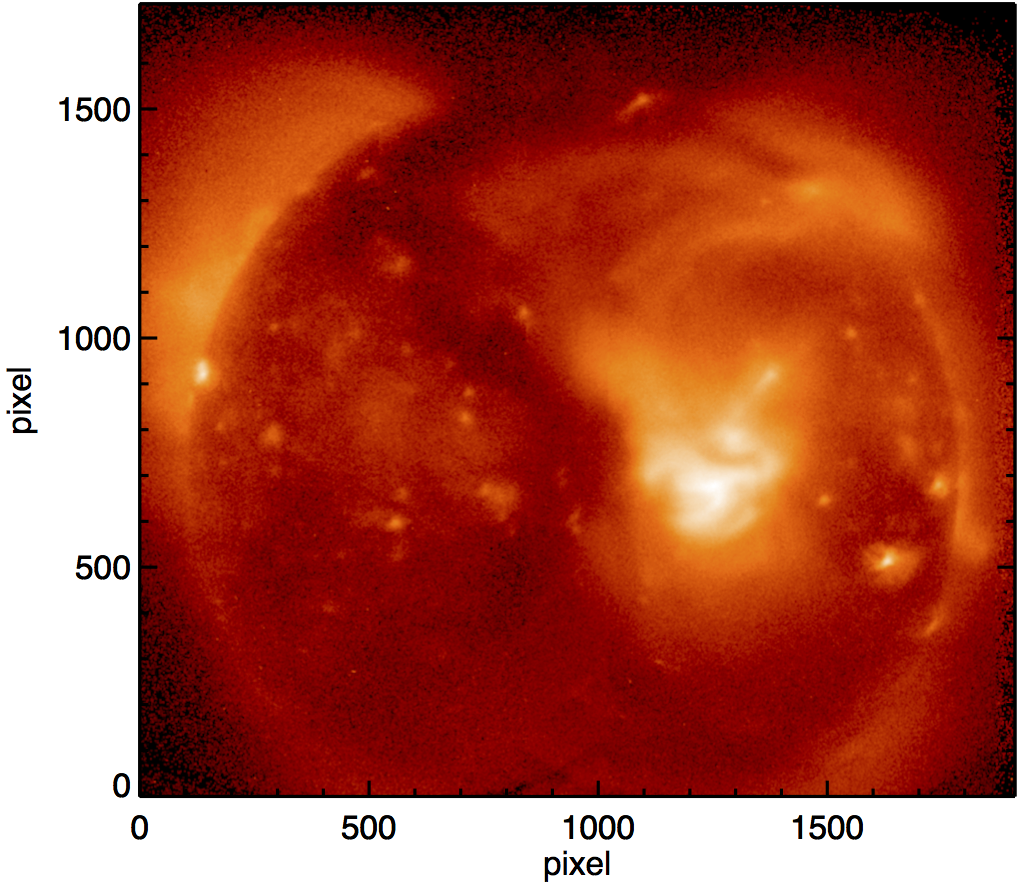
\includegraphics[width=6cm]{foxsi3-full-sun.png}
\caption{FOXSI-3 phoenix full sun soft X-ray image \cite{weko_20796_1}}
\label{fig:foxsi-fullsun-image}
\end{figure}

\subsection{Wolterミラーの設計}
\label{chap1_wolter_arrangement}
FOXSI4に搭載予定のX線用Wolterミラーは、放物面、双曲面の順に反射するI型に分類される。

表\ref{tb:wolter_params}は、開発対象のWolter I型のミラー設計パラメータを図\ref{fig:wolter_params}に対応させて示したものである。

\begin{figure}[h!]
\centering
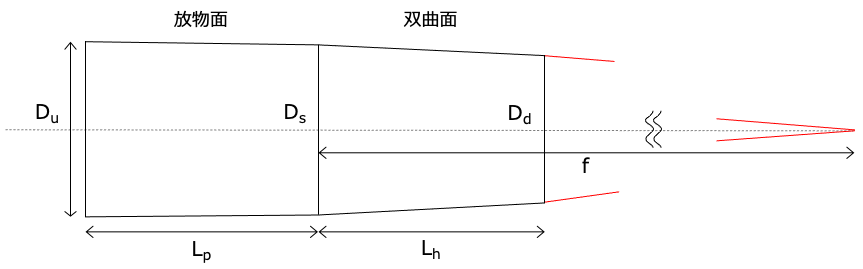
\includegraphics[width=12cm]{wolter_mirror_params.png}
\caption{Wolterミラーの設計変数}
\label{fig:wolter_params}
\end{figure}

\begin{table}[ht]
\begin{center}
  \caption{Wolterミラー各設計変数の値}
  \begin{tabular}{|c|c|l|} \hline
    変数 & 値 & 説明 \\ \hline
    $d_u$ & 60.801 mm & 上流端開口直径 \\
    $d_s$ & 60.000 mm & 接合部直径 \\
    $d_d$ & 57.689 mm & 下流端開口直径 \\
    $l_p$ & 102.501 mm & 放物面部長さ \\
    $l_h$ & 97.499 mm & 双曲面部長さ \\
    $ml$ & 200.000 mm & ミラー全長 \\
    $f$ & 2000.000 mm & 焦点距離 \\ \hline
  \end{tabular}
  \label{tb:wolter_params}
\end{center}
\end{table}

これらを図\ref{fig:wolter_profile}のように放物面部および双曲面部の設計半径として表すと、下式(パラメータは図\ref{tb:wolter_profile_constants})のようになる。
$f1$は座標系の平行移動に関して任意であるため、変数として表記する。

\begin{equation}
    r_p(z) = \sqrt{ -4p(z - p - f_2) } \\
\end{equation}

\begin{equation}
    r_h(z) = b \sqrt{ \frac{(z - (f_1 + f2) / 2)^2}{a^2} - 1.0 }
\end{equation}

\begin{figure}[h]
\centering
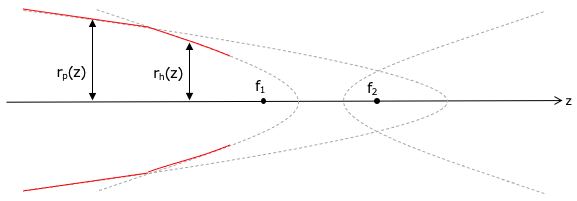
\includegraphics[width=10cm]{mirror_profile.png}
\caption{Wolterミラーの設計半径}
\label{fig:wolter_profile}
\end{figure}

\begin{table}[htb]
    \begin{center}
      \caption{Wolterミラーの設計半径における定数}
      \begin{tabular}{|c|c|l|} \hline
        定数 & 値 & 説明 \\ \hline
        $p$ & 0.0562 mm & 下流端開口直径 \\
        $a$ & 1000.056 mm & 放物面部長さ \\
        $b$ & 10.606 mm & 双曲面部長さ \\ 
        $f_1$ & 任意 & 焦点座標 \\
        $f_2$ & $f_1 + 2 \sqrt{ a^2 + b^2 }$  & 共焦点座標 (双曲線のもう一方の焦点) \\\hline
      \end{tabular}
      \label{tb:wolter_profile_constants}
    \end{center}
\end{table}


\subsection{マンドレル電鋳法}
\label{chap1_mirror_mandrel}

ここで、測定対象となるWolterミラーの製造プロセスについて述べる。
凹状になっている回転体形状のミラー内面を高精度に加工することは難しく、凸形状のマンドレルを高精度に加工し、これに対してさらに転写加工を行うという手法が提案されている。\cite{Mimura2018}
図\ref{fig:mandrel_plating_pictures}に回転楕円ミラーに対するマンドレル電鋳法の一連の流れを示す。

\begin{figure}[!ht]
\centering
\subfloat[高精度に加工されたマンドレル]{
    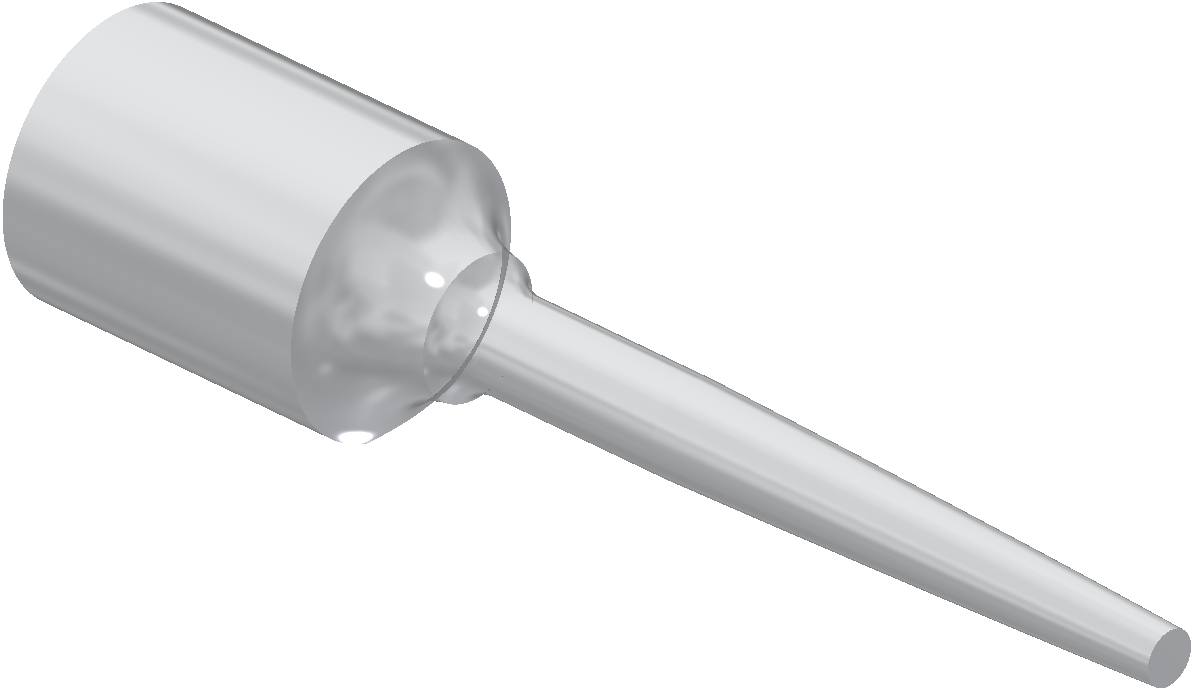
\includegraphics[width=4cm]{mandrel_before_plating.png}
    \label{fig:mandrel_before_plating}
}
\subfloat[マンドレルに転写されたミラー]{
    \centering
    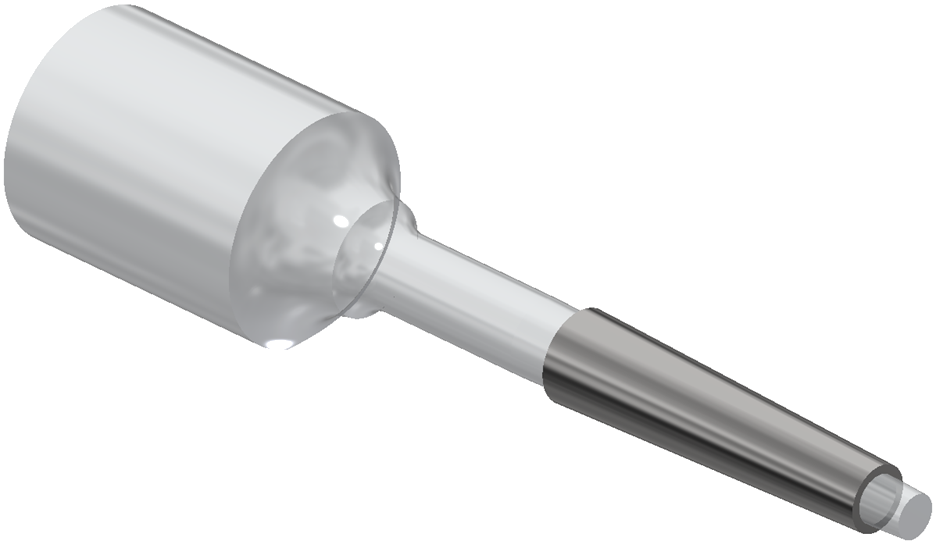
\includegraphics[width=4cm]{mandrel_after_plating.png}
    \label{fig:mandrel_after_plating}
}
\subfloat[取り外されたミラー]{
    \centering
    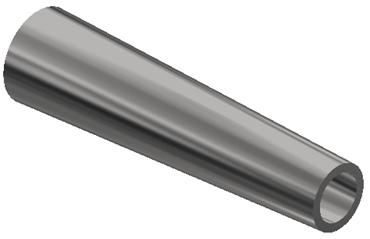
\includegraphics[width=4cm]{detached_mirror.png}
    \label{fig:detached_mirror}
}
\caption[]{マンドレル電鋳法の模式図}
\label{fig:mandrel_plating_pictures}
\end{figure}

I型のWolterミラーは同様の手法による加工が可能であり、既に真円度誤差\SI{20}{\micro \metre}程度以下の精度で作製されている。\cite{Yamaguchi2020}

\subsection{直接計測法}
\label{chap1_direct_measurement}

久米らは、図\ref{fig:profile_measurement_schematic}および図\ref{fig:profile_measurement}に示すように、中空形状のミラー内面に対して接触式変位計を用いて周方向および長手方向の形状誤差プロファイルを取得し、これらを組み合わせることにより3次元形状の決定を試みた。\cite{Kume2017}
しかし、このような計測手法で測定されるのはある始点からの変位量のみであり、直径や長手プロファイルの傾き(テーパ角)といった絶対値の情報を得ることができない。
また、長手方向の計測において始点の位置出しは難しく、中心軸の湾曲など長周期の形状誤差を測定できない。
ミラーの結像性能を悪化させる要因を特定し作製過程へのフィードバックを行うためには、このような誤差プロファイル計測では得られない情報を補完する計測方法が必要である。
また、高精度に加工されたミラー内面に対する計測においては、表面形状を悪化させる恐れのない非接触式の計測方法が好ましい。

\begin{figure}[h]
\centering
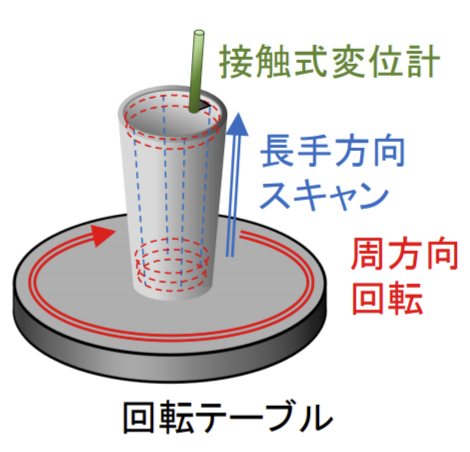
\includegraphics[width=5cm]{profile_measurement_schematic.png}
\caption{接触式誤差プロファイル計測}
\label{fig:profile_measurement_schematic}
\end{figure}

\begin{figure}[!ht]
\centering
\subfloat[長手方向形状]{
    \centering
    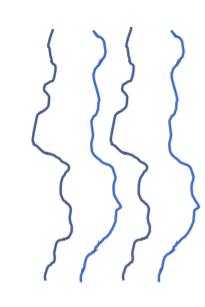
\includegraphics[height=4cm]{meridional_profile.png}
    \label{fig:meridional_profile}
}
\subfloat[周方向形状]{
    \centering
    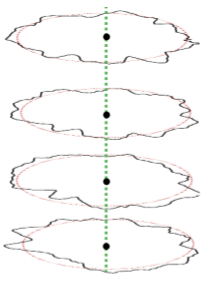
\includegraphics[height=4cm]{sagital_profile.png}
    \label{fig:sagital_profile}
}
\subfloat[3次元形状]{
    \centering
    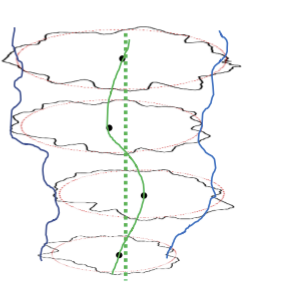
\includegraphics[height=4cm]{combined_profile.png}
    \label{fig:combined_profile}
}
\caption[]{プロファイル計測による3次元プロファイルの構成}
\label{fig:profile_measurement}
\end{figure}


\clearpage
% -------------------------------------------------- %
% section
% -------------------------------------------------- %
\newpage
\section{波面計測法によるミラー形状の解析}
\label{chap1_wave_metrics}

プロファイル計測では得られない情報を取得すること、またネスト構造のミラーを計測可能な間接測定であることという2つの要請を満足させる方法として、波動光学の理論を応用した波面計測法がある。
波動光学では、光を複素スカラー場$U(P)=A(P)\exp(i\Phi(P))$として表現し、等位相面$\Phi(P)=const$を波面とよぶ。
一般に、ある光が1点に収束するとき、その光は収束点を中心とする球面状の波面を持つ。
これに対し、実際の結像系では加工の誤差や設置時の誤差を反映して波面が変形し、その分布と変形量に応じて結像性能が悪化する。
波面計測法では、この波面のずれを波面誤差$\Delta\Phi(P)/k$として求め、結像性能を悪化させる要因を特定しその具体的な量を推定する。

\subsection{測定対象となるWolterミラーの特性}
\label{chap1_wolter_specific_feature}

口径が大きく射入射角の小さいWolterミラーはNAがやや低く、計測するべき集光波動場は図\ref{fig:wolter_thinring}に示すような細い輪帯形状をなす。
口径 60 mm に対して輪帯の幅は\SI{363.3}{\micro \metre}であり、高い空間分解能を実現可能な計測手法が求められる。
波面精度を十分に確保しつつ、空間分解能が十分に高い波面計測法を開発する必要がある。

\begin{figure}[h!]
\centering
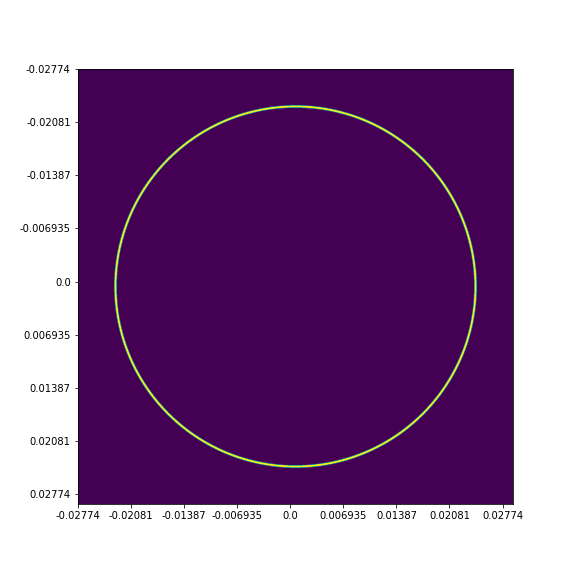
\includegraphics[width=7cm]{wolter_thinring.png}
\caption{Wolterミラー下流端面における集光波面}
\label{fig:wolter_thinring}
\end{figure}

\subsection{可視光による測定}
\label{chap1_visible_light_measurement}

高い空間分解能での測定という要求に加えて、測定装置が実験室内で実現・構成できるようなものであることが望まれる。
波面計測の光源としてX線を利用すれば、より微細な誤差情報を得ることができる。
しかし、波面計測に不可欠なコヒーレンス性の高いX線は限られた施設でしか扱えないため、頻繁に測定実験を行うことは難しい。
FOXSIプロジェクトのような短い期間での性能改善が求められる開発において、計測結果から加工プロセスへのフィードバックはより短いスパンでなされることが期待される。
そのため、本研究では入手性がよく研究や産業用途で広く利用されるHe-Neレーザ(波長 632.8 nm)を光源として用い、よりシンプルな光学配置による計測実験系を構築する。

\subsection{従来的な波面計測法}
\label{chap1_conventional_wave_metrics}
可視光領域での波面計測手法として広く利用されているのが、シャックハルトマンセンサである。
シャックハルトマンセンサは図\ref{fig:shack_hartmann_schematic}のように測定する波動場を2次元のレンズアレイに入射させ、集光点の位置ずれをディテクタで検出することによって波面誤差を計測する。
欠点として、球面波による校正が必要であるため、計測手順が煩雑であることが挙げられる。
校正を経た計測であっても、波面の安定性が高いとは言えず、X線ミラーの計測には適さない。
また、レンズアレイの大きさによって空間分解能が制限されてしまうため、Wolterミラーの細い輪帯を計測するのに不向きである。

\begin{figure}[h]
\centering
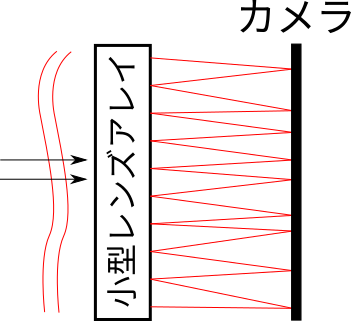
\includegraphics[width=5cm]{shack_hartmann_schematic.png}
\caption{シャックハルトマンセンサ}
\label{fig:shack_hartmann_schematic}
\end{figure}

\subsection{位相回復法}
シャックハルトマンセンサでは、実現するべき空間分解能に対して、素子のサイズが律速となってしまうという問題があった。
これに対して、位相回復法では空間分解能を測定領域の大きさという別の問題に置き換えることができる。
位相回復法とは、測定対象のミラーによって集光されたビームにオブジェクトを差し入れ、背後に現れる回折像の強度分布計測値から繰り返し計算によって位相情報を算出する方法である。
この手法の背景には、集光光学系における波動場の伝播がFourier変換の関係で与えられるという物理的法則がある。
Fourier変換の関係で結ばれる2つの波動場は、互いにもう一方の周波数領域での表現となる。
ゆえに、伝播先の波動場を広い範囲で測定することは、元の波動場の高周波の情報を得ることに対応する。
このことを利用すれば、計測面における空間分解能を上げるという問題を、焦点面における測定領域を広げるという問題に置き換えることができる。
位相回復法を用いることで、測定装置を構成する素子の最小サイズによって制限されることなく、空間分解能の高い測定が可能となる。
本研究では、位相回復法を採用し、また位相回復法の中でもより高い空間分解能が実現される形状測定装置の構成について検討する。

\clearpage
% -------------------------------------------------- %
% section
% -------------------------------------------------- %
\newpage

\section{本論文の目的および構成}
\label{chap1_purpose}

ここまで、X線天文学における結像用Wolterミラーの有用性、およびFOXSI4に搭載されるWolterミラーの測定に用いる装置に求められる要件について述べた。
本研究では、\ref{chap1_wave_metrics}節で述べたように可視光光源を用いた位相回復法による計測装置の提案および検証実験を行う。
まず、\ref{chap3}章で様々な位相回復法について検討し、計測に用いる手法を提案した上で、シミュレーションにより手法の正当性を検証する。
\ref{chap5}章では、実際に加工されたFOXSI4用のWolterミラーに対して計測実験を行い、その結果について考察する。
最後に、\ref{chap6}章で考察、結論および今後の展望について述べる。

%%%%%%%%%%%%%%%%%%%%%%%%%%%%%%%%%%%%%%%%%%%%%%%%%%%%%%%%%%%%%%%%%%%%%%%%%%%%%
%%% Local Variables:
%%% mode: katex
%%% TeX-master: "../thesis"
%%% End:
